\section{Common Systems}
This section describes systems that are common to the detectors in both
spectrometers.

\subsection{CAEN High Voltage System}

\paragraph{Overview}

The CAEN Distributed High Voltage System is responsible for
providing high voltage power to all HMS and SHMS detector systems
including phototubes for hodoscopes, Cerenkov detectors, and shower
counters as well as wire voltages for drift chambers. 
This system is a
networked system made up of individual crates (Controllers)
each of which can hold several independent high voltage modules
(Cards).  The crates are a mix SY403 mainframes which hold four cards
with 16 SHV outputs and newer SY4527 mainframes holding up to 8 cards with 24
SHV outputs each.  (Other cards with different numbers of channels and
different high voltage connector form factors are available, but only
the described types are used in Hall C.)
There are several flavors of cards in use with the
Hall~C detector systems which are listed in Tables~\ref{tab:hv_cards}
and \ref{tab:hv_cards_new}.  A given crate may have a mix of card
types, although cards can not be exchanged between SY403 and SY4527 crates.

\begin{table}
\caption{Specifications of SY403 High-Voltage Cards used in Hall~C Detector 
Systems\label{tab:hv_cards}.}
\begin{center}
\begin{tabular}{ccccc}
        &Card type      &Max Voltage    &Max Current    &Detector System \\
	&		&		&		&	\\
	& A403 (or A503)&--3000V		&3.0mA		&Hodo/Shower\\
	& A503P		&+3000V		&3.0mA		&Cerenkov/Aerogel\\
	& A505		&--3000V		&200$\mu$A 	&Drift Chambers\\
  \end{tabular}
\end{center}
\end{table}

\begin{table}
\caption{Specifications of SY4527 High-Voltage Cards used in Hall~C Detector 
Systems\label{tab:hv_cards_new}.}
\begin{center}
\begin{tabular}{ccccc}
  &Card type      &Max Voltage    &Max Current    &Detector System \\
  &		&		&		&	\\
  & A1535SN       &--3500V	&3.0mA		&Hodo/Shower/Heavy Gas\\
  & A1535SP       &+3500V    &3.0mA		&Noble Gas/Aerogel\\

  \end{tabular}
\end{center}
\end{table}

The system can be controlled/monitored both locally (by a built-in
display panel on the individual Crates) or remotely by either a
connected Terminal (RS232) or VME CAEN net interface card (Model V288).


\begin{figure}
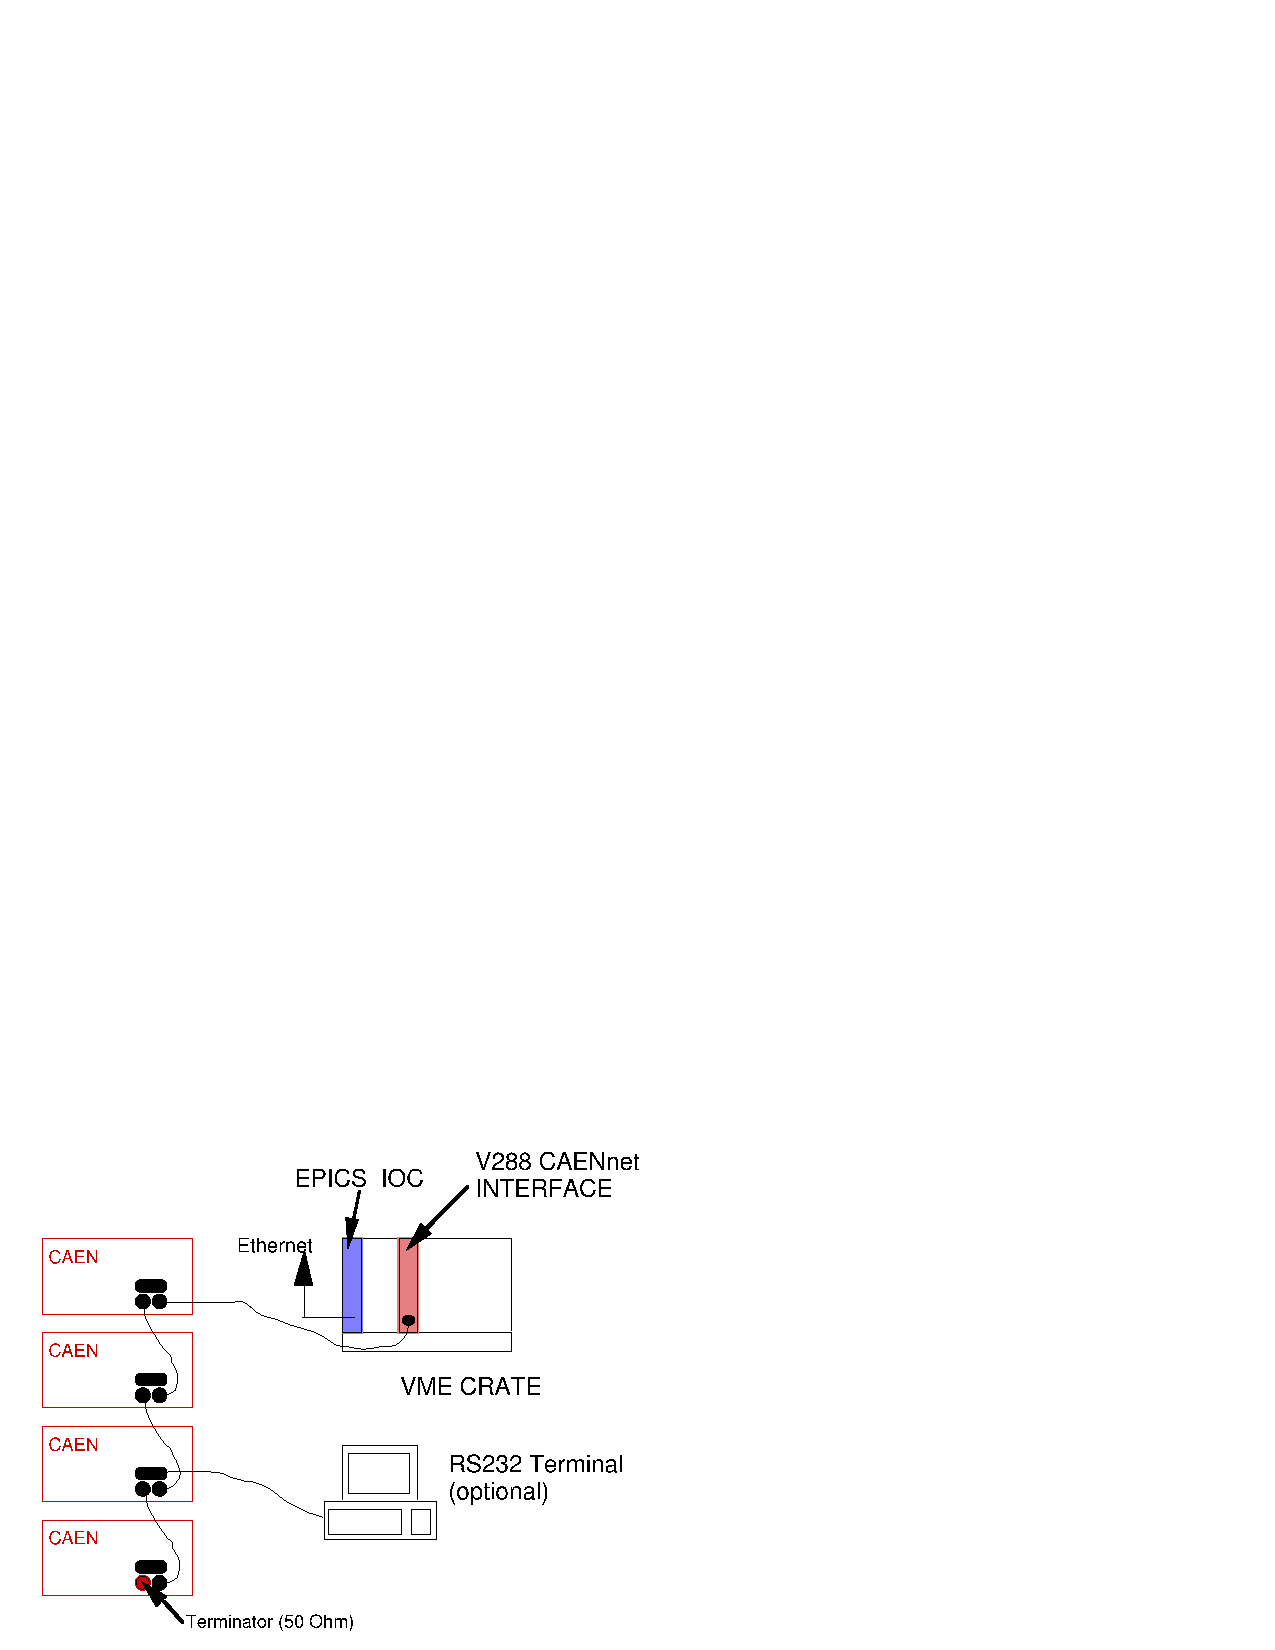
\includegraphics[height=4.5in]{CAENHV.pdf}
\caption{Generic CAEN High Voltage System setup\label{fig:caen_setup}}
\end{figure}

HV channel assignments currently in effect are indicated in 
two files ("group\_map" and
"channel\_map") in the directories \$EPHHV/perl (for HMS) and \$EPSHV/perl (for
SOS) when you are logged in as cvxwrks to one of the cdaq machines.

%\vfil\eject
\paragraph{General Operation}

\subparagraph{Normal Operation:}

In general the high voltage system will be controlled or monitored
from the counting house using the EPICS slow control system which will
be interfaced through a V288 card located in a VME crate in rack CH03B13
in the electronics room of the counting house
(see Figure~\ref{fig:caen_setup}).  It is also possible, but not recommended,
to control a CAEN crate using its front panel display or a terminal
if one is connected to the crate.
For EPICS control/monitoring all crates must be interconnected with 50
ohm (terminated) cable and all crates must be powered on whether they
will be in use or not.

Configuration of individual HV output channels is done through a
text file which is read in and downloaded when EPICS control is
configured. Step by step instructions for modifying this file and
reconfiguring the system are provided in the document
\htmladdnormallink{$\sim$cdaq/documents/slow\_controls/hvcntl.text}{http://www.jlab.org/Hall-C/document/slow_controls/hvcntl.text}. Do the HV rebuilds on cdaqs1 as cvxwrks.


It is imperative that
you follow the steps as shown there and not try to invent your own
procedure.
All relevant parameters
can be programmed through this interface.  The user must only know the
Crate Numbers and the Channel Numbers that his equipment is connected
to.  The crate number can be gotten from the front panel display and the
channel numbers run from 0-63 for each crate ( If only three cards are
installed, the channel number will run from 0-47 top to bottom
regardless of their positions in the crate).

\subparagraph{Important Features:}

The user can program several important features for individual
cards and/or channels.  The most common are:

\begin{itemize}
\item{HV limits -- 2 types including a hardware maximum (common to a
card) set with a pot on the front panel of each card and a software
maximum for each channel.}
\item{Current Trip Value -- The current over which the system will
indicate an alarm status and initiate a trip off of that channel.}
\item{Current Trip Time -- The amount of time the system will allow
the alarm condition before actually switching off that channel.}
\item{Ramp-up Value -- The number of volts/sec the voltage will ramp
to its set point upon switching on the channel.}
\item{Other Features -- See the CAEN Technical Information Manual.}
\end{itemize}

\subparagraph{Remote Operation: the High Voltage GUI system}
Remote operation of the CAEN system is described in the section
\ref{par:hv_ops}.

\subparagraph{Local (Front Panel) Operation}

Modifications to the parameter settings should in general not be
made at the front panel or through a locally connected terminal if the
EPICS system is in operation.  This mode of control is meant for
diagnostics and testing of a detector system prior to running.  There is
only one feature which must be set at the front panel before initiating
an EPICS control session - this is the crate number.  The RS232
parameters must also be set from the front panel ( suggested default are
9600 baud  no parity  1 stop bit).

If unfamiliar with the operation of the HV system in local modes
one should get experienced personnel or review the CAEN Technical
Information Manual.

\paragraph{Safety Concerns/Caveats}

There are a number of cautions one should observe when operating
the CAEN HV equipment to avoid damage and insure proper functioning:

\begin{itemize}
\item{Use only proper SHV connectors and approved cables when
connecting equipment to the supply.}
\item{{\bf DO NOT} attach/remove HV cables when loads are present on the
channel ( a red LED above each channel indicates the presence of a
load).}
\item{Insure adequate ventilation around crates to avoid overheating
of the electronics.}
\item{Wait 2-3 minutes after switching off a crate before removal of a
HV card.}
\item{Insure proper static precautions when handling HV cards.}
\end{itemize}

For proper EPICS control operation:

\begin{itemize}
\item{Inter-crate connections must be unbroken and terminated at the
last crate at 50 Ohms.  All crates must be powered on.}
\item{Crate numbers for each crate in the chain must be distinct and
different from 0 (i.e. 1-99)}
\item{The HV Enable switch (on the front panel of each crate) must be on.}
\item{One should refrain from any local operation of crates when the
EPICS system is active.}
\end{itemize}

\subsection{The Wire Chamber Gas Mixing System}
% (BDS) Largely pulled from detailed gas_system_HOWTO document

The Hall~C wire chamber gas mixing system exists in the gas shed located
to the left of the counting house in the parking lot between the counting house
and the accelerator service building (building 96C).  The main
component of the system is a single MKS 647 menu driven 4-channel
controller that maintains the mix proportions and pressure regulation of the
gas supplied to the wire chambers.  Gas flow is
controlled by 2259c proportional mass flow control valves.  The 647 allows
the Gas Calibration factor to be altered in software, allowing the user to
change to a different gas without recalibration of the mass flow control
valves.

A temperature controlled alcohol bubbler is provided for the gas
stream.  The alcohol level in the stream is maintained by a float valve
fed from a reservoir outside the bubbler chiller. This allows the alcohol
system to be refilled without opening the system to air.  A sight glass on
the side of the reservoir allows the level to be monitored.  A bypass loop
around the alcohol system is provided should alcohol-free gas be desired,
or if the alcohol system requires maintenance.  Remote monitoring and limited
controls are provided through an EPICS display screen accessible via
\textbf{JMenu/Monticello $\rightarrow$ Hall C $\rightarrow$ Hall C Gas Shed},
or equivalent\footnote{Path to EDM file is /cs/opshome/edm/hlc/HLC\_gas\_shed.edl}.

{\bf This system operates by measuring and controlling pressure, not flow rate.
This system will work to maintain a pressure, regardless of the flow rate.
This allows the (pressure dependent) Rotameter-style flow meters to provide
a constant flow rate to detector systems.  Nevertheless, it should not be used
without appropriate pressure relief device such as relief bubblers and relief
valves.}

The manual valves used in this system are numbered on their
handles.  Those numbers are referenced in this document and in
Figure~\ref{fig:gas_mix}.
\begin{figure}
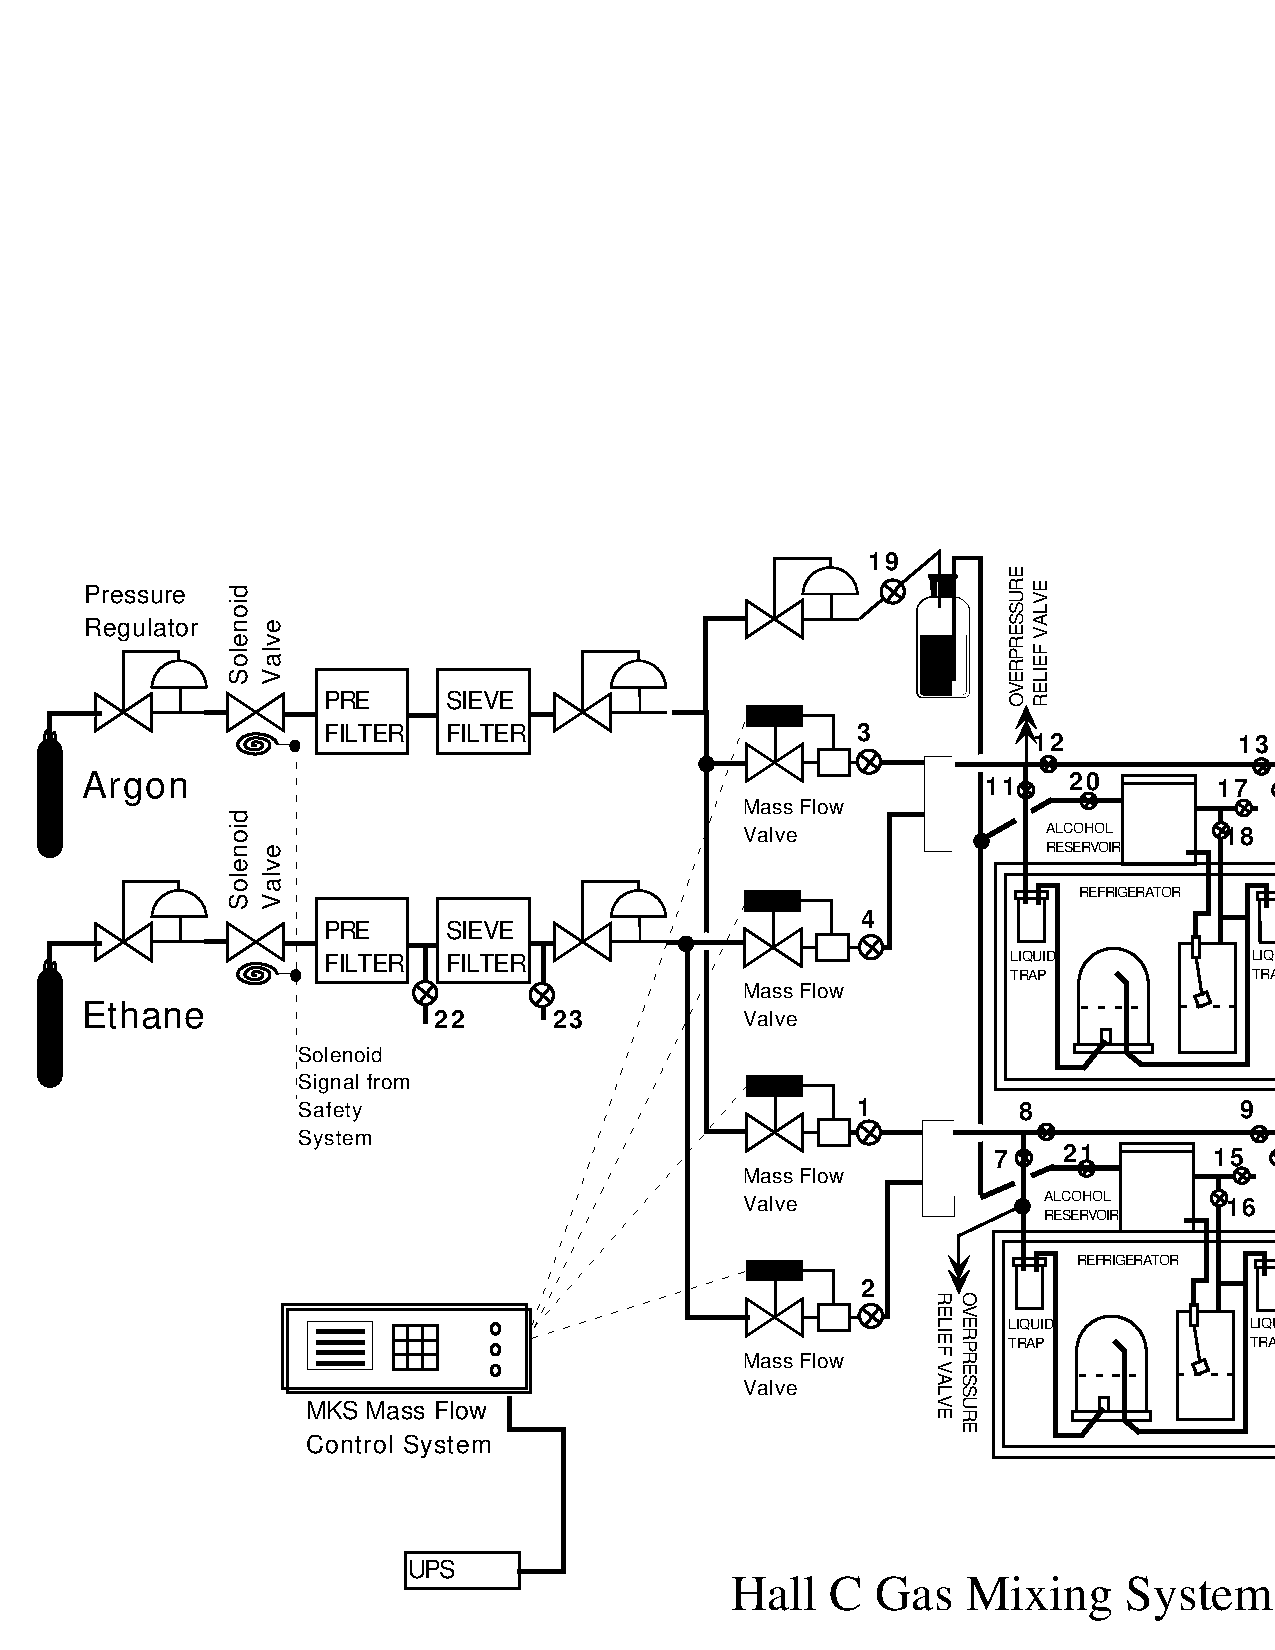
\includegraphics[width=0.9\columnwidth]{HallCGasMixlvl1.pdf}
\caption{Diagram of the Hall~C Gas Mixing System\label{fig:gas_mix}}
\end{figure}

\paragraph{Settings for Normal Operation}

A summary of all of the settings required to make the controller
function properly is given in Table~\ref{tab:mixer_nominals}. The
table also shows which screen contains each parameter. Instructions
for setting parameters are given below. Detailed instructions for
configuring and operating the MKS~647 can be found in the
manufacturer's instruction manual, a copy of which is posted at
\url{https://hallcweb.jlab.org/document/vendor\_manuals/}.

\begin{table}[hbt]
\begin{minipage}[h!]{\textwidth}
{\scriptsize
\begin{center}
\begin{tabular}{|l|c|l|}
\hline
Parameter   & Set To   & {\it Controller Screen}/Comments\\ \hline
\multicolumn{2}{|c|}{\bf Manual Valves  } &  Valves are labeled        \\
Valves 1, 2, 4, 8 & OPEN                  &         \\
Valves 3, 5, 6, 7 & CLOSED                &         \\ \hline
\multicolumn{2}{|c|}{\bf Pressure PID Loop Settings   } & {\it Pressure Control} (Fig. \ref{fig:pressure_control})  \\
Pressure    & 500 Torr &                   \\
PID Mode    & AUTO     &                   \\
PID GAIN    & 4.0      &                   \\
PID INTEG   & 10.0     &                   \\
PID LEAD    & 0.000    &                   \\ \hline
\bf Mixture     & 1        & {\it User} (Fig. \ref{fig:user_display})/ Lower-right corner\\ \hline
\multicolumn{2}{|c|}{\bf Gas Composition for Mixture 1} & {\it Gas Composition} (Fig. \ref{fig:gas_composition})\\
Channel 1   & 1.000    &  (Argon)                 \\
Channel 2   & 1.000    &  (Ethane)                 \\
Channel 3   & 0.000    &                   \\
Channel 4   & 0.000    &                   \\ \hline
\multicolumn{2}{|c|}{\bf MFC Valve Size } & {\it Range Selection} (Fig. \ref{fig:range_selection})  \\
\multicolumn{2}{|c|}{\bf  / Gas}             & {\it Gas Selection} (Fig. \ref{fig:gas_selection})  \\
Channel 1   & 2.0 SLM / Ar         & provides 2.78 SLM Argon\\
Channel 2   & 5.0 SLM / C$_2$H$_6$ & provides 2.50 SLM Ethane\\
Channel 3   & \it unused&                  \\
Channel 4   & \it unused&                  \\ \hline
\multicolumn{2}{|c|}{\bf Channels ON/OFF Settings} & {\it Extended Display} (Fig. \ref{fig:extended_display})   \\
Channel 1   & ON       &                   Press ``ON 1'' (\em Argon)  \\
Channel 2   & ON       &                   Press ``ON 2'' (\em Ethane) \\
Channel 3   & OFF      &                   Press ``OFF 3'' (\em not in use) \\
Channel 4   & OFF      &                   Press ``OFF 4'' (\em not in use) \\ \hline
\multicolumn{2}{|c|}{\bf Pressure Transducer} & {\it Pressure Setup}  \\
Controller  & STD      &                   \\ 
Range F.S.  & 1000 Torr&                   \\ \hline
\multicolumn{2}{|c|}{\bf MFC Valve Controls     } & {\it Mode Selection} (Fig. \ref{fig:mode_selection}) \\
Channel 1   & PID      &                                   \\
Channel 2   & SLAVE / 1&                                   \\
Channel 3   & INDEP    &                                   \\
Channel 4   & INDEP    &                                   \\ \hline
\bf Alcohol Temp. & 2$^\circ$\,C & Electronic Temperature  \\
                  &              & Control Box             \\ \hline
\hline
\end{tabular}
\end{center}
}%end of \scriptsize
\end{minipage}
\caption{Normal Valve and Parameter Settings for the Gas Mixing System.
\label{tab:mixer_nominals}}
\end{table}
%=====================================================================
\paragraph{General Operation of the Mass Flow Controller}
If the controller screen is dark, press {\bf ESC} to awaken the
display.  Many screens merely provide a menu of other screens you may
access: simply press the item number you desire. To go up one level in
the menu hierarchy, press {\bf ESC}. The \emph{Menu Tree} for the 647C
controller is shown in Fig. \ref{fig:command_tree}.

In general, to change a parameter displayed on the controller screen
use the \textbf{left/ right} arrow keys to move the cursor to the item you
wish to change. Then either use the number keys to enter the value
desired for that item (numeric parameter) or use the {\bf ENTER} or
{\bf up/down} keys to cycle a parameter through its available settings
(configuration parameter). Numeric parameters may be incrementally
modified by using the {\bf up/down} arrow keys. To make certain that a
new parameter becomes active, move the cursor off of the parameter
after you have entered the new value.

The initial menu upon startup is the {\bf Main Menu}
(Fig.~\ref{fig:main_menu}).  For normal operation use the {\bf User
Display} menu (Fig.~\ref{fig:user_display}). It shows the amount of
each gas currently flowing, the total gas flow, and the current
delivery pressure. This display also shows which of several possible
pre-defined gas mixtures is selected. These mixtures are configured 
on the {\bf Gas Composition} screen, Fig. \ref{fig:gas_composition}.
For normal operation, we use
only mixture {\bf \#1}, (number shown on the lower-right of the
display). {\bf Only on this screen can this parameter be changed.}
Mixture {\bf \#2} is usually configured to provide 100\% argon for
purging flammable gas out of the chambers.

The {\bf Extended Display} menu (Fig.~\ref{fig:extended_display})
shows actual flow, flow set point, units, valve full-scale range, gas
calibration factor, whether that channel is enabled, and whether each
channel is operating in master, slave, PID, or independent mode. This
display is most useful to a system expert wishing to verify the system
parameter settings.  Most parameters cannot be modified from this
screen, however.

Delivery pressure set-point and pressure \emph{PID-loop} control parameters
may be configured from the {\bf Pressure Control} screen
(Fig.~\ref{fig:pressure_control}).
%
\begin{figure}[tb]
\begin{center}
\framebox{
\begin{minipage}{.65\textwidth}
\footnotesize
\begin{itemize}
\item MAIN MENU (Fig. \ref{fig:main_menu})
   \begin{enumerate}
   \item [1] USER DISPLAY (Fig.\ref{fig:user_display})
   \item [2] EXTENDED DISPLAY (Fig.~\ref{fig:extended_display})
   \item [3] PRESSURE CONTROL (Fig.~\ref{fig:pressure_control})
   \item [4] DIAGNOSTICS
      \begin{enumerate}
      \item [4.1] ERROR LISTING
      \item [4.2] SIGNALS
      \end{enumerate}
   \item [5] INSTRUMENT SETUP
      \begin{enumerate}
      \item [5.1] RANGE SELECTION (Fig.~\ref{fig:range_selection})
      \item [5.2] GAS SELECTION (Fig.~\ref{fig:gas_selection})
      \item [5.3] MODE SELECTION (Fig.~\ref{fig:mode_selection}) 
      \item [5.4] ZERO ADJUST
      \item [5.5] TRIP LIMITS
      \item [5.6] GAS COMPOSITION (Fig.~\ref{fig:gas_composition})
      \end{enumerate}
   \item [6] SYSTEM SETUP
   \item [7] PRESSURE SETUP 
   \item [ ]
   \item [9] INFORMATION
   \item [0] POWER OFF
   \end{enumerate}
\end{itemize}
\end{minipage}
} %%end of \framebox{
\caption{Command Tree for the MKS-647C Control Panel}
\label{fig:command_tree}
\end{center}
\end{figure}
%
\begin{center}
\begin{figure}[hbt]
\begin{minipage}{2.7in}
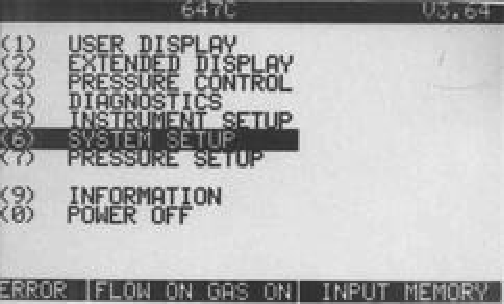
\includegraphics[width=2.6in,height=1.8in]{drift_gas_system-main_menu-eps-converted-to.pdf}
\caption{MKS~647 Main Menu\label{fig:main_menu}}
\end{minipage}
\begin{minipage}{2.7in}
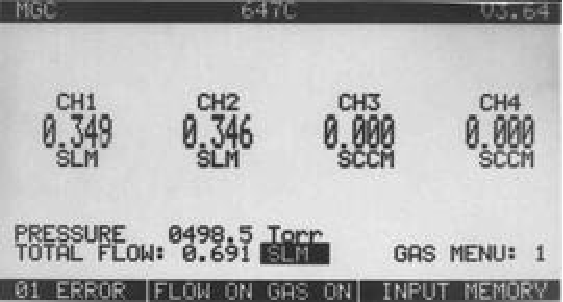
\includegraphics[width=2.6in,height=1.8in]{drift_gas_system-user_display-eps-converted-to.pdf}
\caption{MKS~647 User Display\label{fig:user_display}}
\end{minipage}
\end{figure}
\end{center}
%
\begin{center}
\begin{figure}[hbt]
\begin{minipage}{2.7in}
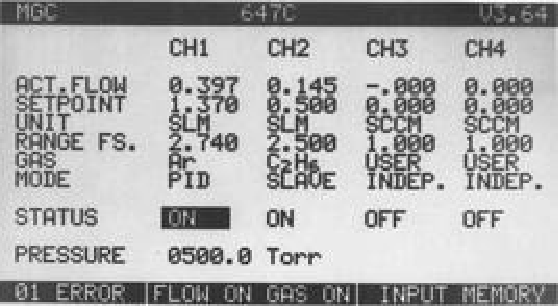
\includegraphics[width=2.6in,height=1.8in]{drift_gas_system-extended_display-eps-converted-to.pdf}
\caption{Extended Display Screen\label{fig:extended_display}}
\end{minipage}
\begin{minipage}{2.7in}
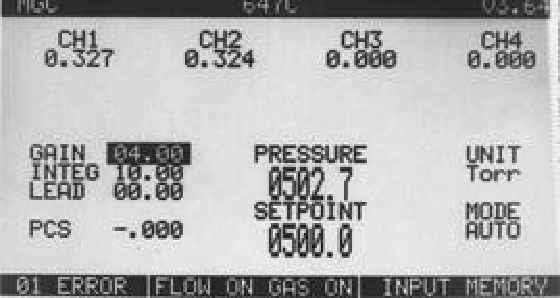
\includegraphics[width=2.6in,height=1.8in]{drift_gas_system-pressure_control-eps-converted-to.pdf}
\caption{Pressure Control Screen\label{fig:pressure_control}}
\end{minipage}
\end{figure}
\end{center}
%=====================================================================
\paragraph{Gas Flow Rates}
\label{sec:gas_flow_rates}
The flow rates are adjusted automatically by the controller in order
to maintain a constant delivery pressure at the output. Only the flow
{\em ratios} should be set by the operator. We use a 1:1 ratio, set on
the {\bf Gas Composition} screen (Fig.~\ref{fig:gas_composition}), as
indicated in Table~\ref{tab:mixer_nominals}.

The average total flow should equal the sum of the flows to all of the
detectors in the shield house. (Note that the ball-type flowmeters in
the shield house are calibrated for nitrogen. The approximate
multiplier to convert these readings for 50/50 Argon-Ethane is 0.9 .)

System configuration parameters specifying the full-scale flow
capacity (for nitrogen) of each valve, the types of gases actually
flowing through each valve, and the mode of control for the valves are
set in the screens pictured in Figs.~\ref{fig:range_selection},
\ref{fig:gas_selection}, and \ref{fig:mode_selection}. These figures
show the nominal settings for the Hall-C system.

\begin{center}
\begin{figure}[hbt]
\begin{minipage}{2.7in}
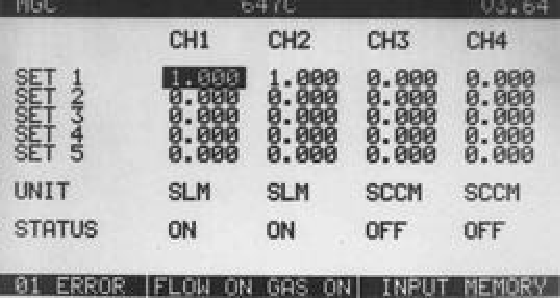
\includegraphics[width=2.6in,height=1.8in]{drift_gas_system-gas_composition-eps-converted-to.pdf}
\caption{Gas Composition Screen\label{fig:gas_composition}}
\end{minipage}
\begin{minipage}{2.7in}
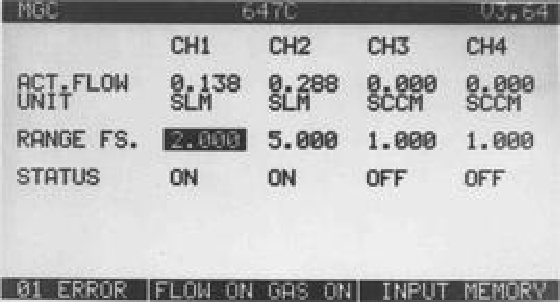
\includegraphics[width=2.6in,height=1.8in]{drift_gas_system-range_selection-eps-converted-to.pdf}
\caption{Range Selection Screen\label{fig:range_selection}}
\end{minipage}
\end{figure}
\begin{figure}[hbt]
\begin{minipage}{2.7in}
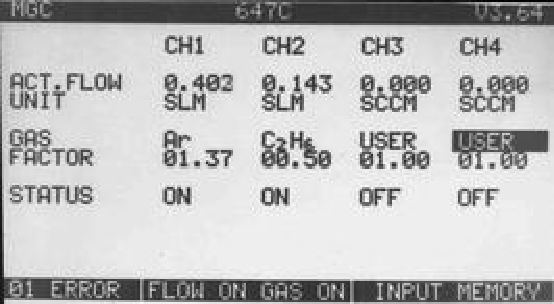
\includegraphics[width=2.6in,height=1.8in]{drift_gas_system-gas_selection-eps-converted-to.pdf}
\caption{Gas Selection Screen\label{fig:gas_selection}}
\end{minipage}
\begin{minipage}{2.7in}
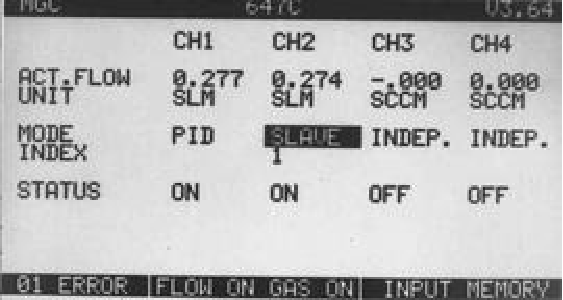
\includegraphics[width=2.6in,height=1.8in]{drift_gas_system-mode_selection-eps-converted-to.pdf}
\caption{Mode Selection Screen\label{fig:mode_selection}}
\end{minipage}
\end{figure}
\end{center}

%=====================================================================
\paragraph{To set the Delivery Pressure:}

Navigate to the {\bf Pressure Control} menu. The pressure set-point (in
Torr) is indicated at the bottom-center of the screen. This value
should be set to 500.0. Note that the system can not respond instantly
to a change in requested gas pressure: it has no way to release excess
pressure and must wait for the detector systems to consume it
\footnote{An \emph{over-pressure relief valve} releases gas through a
small oil bubbler in the gas shed if the pressure exceeds about
600~Torr.}; it cannot build up pressure any faster than the
flow-control valves can supply it. It may take thirty minutes or so
for the pressure regulation system to stabilize at a new set-point or
stabilize in response to a change in total gas consumption. However,
you should be able to observe a change in the gas flow within a few
seconds (possibly up to a minute) after a set-point change.

%=====================================================================
\paragraph{To turn gas flow on or off:}

The gas flow can be turned on or off while in any menu.  In the
Extended Display menu the bottom line displays ``ON'' or ``OFF'', by
channel, to show which mass flow valves are enabled.  ``ON'' must be
displayed in the bottom row of the Extended Display menu for gas to be
flowing in a particular channel.

For gas to flow, two conditions must be met: 
\begin{enumerate}
\item Each channel (1 and 2) must be enabled by pressing ``ON'' and then the
  desired channel number.
\item The entire system must be enabled by pressing ``ON" and then ``ALL" from
  the keypad.
\end{enumerate}
Thus, each valve can be controlled individually using ``ON/OFF~-~\emph{Channel
Number}'', or all flow can be controlled using ``ON/OFF~-~ALL''. If the system
is enabled, the status line at the bottom of every screen will indicate ``FLOW
ON GAS ON''. {\bf Note:} because Valve-2 (ethane) is normally slaved to Valve-1
(argon), when Valve-1 is disabled there will be no flow through Valve-2.

%=====================================================================
\paragraph{To Change a Gas Bottle}

The argon and ethane supply bottles should be replaced by new (full)
bottles when the bottle content drops below about 10\% of its
capacity.  For argon, the bottle content is directly indicated by the
bottle pressure: a new bottle usually contains 2000 to
3000~psig. Argon bottles should be changed whenever the bottle
pressure is found to be below about 200~psig. 

Ethane bottles, on the
other hand, contain liquefied ethane. Thus the bottle pressure is just
the vapor pressure of ethane at whatever the current temperature
happens to be. At 70$^\circ$\,F this is about 544~psig. The pressure gauge
will not tell you how much ethane is left in the bottle until it reads
zero! Instead, we measure the ethane content by observing the weight
of the bottle and comparing it to the weight when the bottle was
full. A standard B-size cylinder contains about 32~pounds of ethane.
The ethane cylinders on the manifold sit on scales which have been 
pre-set to indicate the net weight of ethane in the bottle.
Numbers in the green portion of the dial indicate ethane remaining.
If the indicator points to the red portion of the dial, the bottle
is empty.

Handling and connecting bottles of compressed gas require special
knowledge.  The high pressure gas stored in the cylinders (bottles)
constitutes significant stored energy. Mishandling of a gas bottle can
pose a lethal hazard! Refer to the JLab ESH\&Q Manual
for safe handling practices. If you do not already know how to safely
manipulate compressed gas hardware, have a knowledgeable person train
you.

After attaching a new gas bottle to the supply manifold, check the
connection for leaks using \emph{Snoop} or a similar leak detector.

%=====================================================================
\paragraph{The Alcohol Bubbler}

To reduce the rate of aging of the wire chambers, the operating gas
contains a small quantity of alcohol vapor. The vapor is added by
bubbling the argon/ethane mixture through liquid alcohol. The
temperature of the alcohol controls the alcohol vapor pressure, which
determines the amount of vapor added to the gas. The alcohol content
also affects the electron drift velocity in the wire chambers, so it
must be held approximately constant.

Gas is bubbled through the liquid alcohol inside the glass
dome vessel in the refrigerator. The dome is covered by a
perforated steel cylinder as a precaution against breakage. The
alcohol level is controlled by a float valve inside the metal cold
reservoir, which is also inside the refrigerator. As long as there is
alcohol in the warm reservoir (sitting on top of the refrigerator),
the liquid levels inside the refrigerator will remain constant. A
drain valve (\#7) inside the refrigerator is available for emptying
all liquid from the system.  It is for use by experts only and should
remain closed during normal operation.

%=====================================================================
\subparagraph {Alcohol Temperature Control}

To keep the alcohol temperature (and thus the vapor pressure) constant,
the alcohol bubbler is housed in a refrigerator which is controlled by
an electronic temperature regulator having 1$^\circ$C sensitivity. The 
controller is located on a shelf in the right-hand rack of the gas mixing
system. Normally, the actual temperature in the refrigerator is
indicated on the front panel of the controller. The controller should
be set to maintain a temperature of 2$^\circ$\,C.


%=====================================================================
\subsection{Hall C Laser Pulser System}
The Hall C laser pulser sytem provides light pulses
in the visible  blue scintillation region to monitor
the gain stability of the HMS and SOS shower counters and scintillators,
and, at a later stage, the neutron detector of the $G_{En}$ experiment.

\paragraph{UV Laser System}
We use a nitrogen Laser that provides UV laser pulses at 337 nm
from 1 to 50 Hz repetition rate. The output power is 250 $\mu$J.
It is located in a designated area in the Counting House of Hall C.
The laser is enclosed in an aluminum box where the laser light is directed
onto a scintillation fiber after passing through two optical filters
to optimize the light output. 
The laser light is absorbed in the scintillation fiber
and converted to visible blue scintillation light. Both ends of the
scintillation fiber are coupled using CT connectors, mounted on an
aluminum casing, to regular
1 mm diameter multimode plastic optical fibers. One fiber output is
connected to a PIN diode to monitor the light output; the other
fiber is brought downstairs into Hall C where it is connected to 
a distribution box (1:24) located in the cupboard below the pivot. From
this distribution box 4 fibers are running to the HMS spectrometer and
4 to the SOS spectrometer, where they
are connected again to distribution boxes (1:64). The individual
outputs of the final distribution box are connected to the scintillators
and lead glass shower counters. The light pulses in the detector
produce a trigger in the data acquisition system and ADC and TDC
information is read out. Normalizing the peak positions of the light 
pulses to the PIN diode ADC value is a tool to monitor the gain of
each photo multiplier tube throughout the experiments.

\paragraph{Laser Operation} 
In order to turn on the nitrogen laser the right half of the top
plate of the aluminum box needs to be removed. Inside the box 
the laser and the optics is mounted on a single aluminum board.
The lasing part of the laser is confined in the left part of the box
with a separation in the central region of the box. Due to this separation
no UV laser light can escape from this left part of the box,
even during operation, so that the user can safely remove and install the
top plate above the right half of the laser casing.
The laser itself has a security key that needs 
to be in a vertical position when the power switch is pressed. After
2 minutes of warmup-time an orange light turns on indicating that
it is possible now to turn the key into its horizontal position.
After this it takes 15 seconds until the laser actually turns on.
In the event of a power failure the laser will turn off and will not
turn on again after power is restored. It is necessary to turn the key
back to its vertical position and to reset the safety system of the laser.
The laser can now be turned on again by switching the key back to its
horizontal position. The pulse frequency of the laser can be regulated by
turning the black knob at the rear of the laser casing.
